\documentclass[a0paper,portrait]{baposter}      %%
\usepackage{relsize}		% For \smaller      %%
\usepackage{url}	                            %%
\usepackage{wallpaper}		                    %%
\usepackage{epstopdf}	                        %% This is the basic preamble of the poster.
\usepackage{amsmath,amsthm, amssymb, latexsym}  %% Authors can add other stylefiles for editing theirs papers.
\usepackage{array,booktabs,tabularx}            %% However, the basic preamble should not be reduced or removed so that the poster template runs smoothly.
\usepackage[font=small,labelfont=bf]{caption}   %%
\usepackage{capt-of}                            %%
\usepackage{indentfirst}
\setlength{\parindent}{2em}                     %%
%%% Global Settings %%%%%%%%%%%%%%%%%%%%%%%%%%%%%%%%%%%%%%%%%%%%%%%
\graphicspath{{pix/}}	% Root directory of the pictures         %% Do not change.
\tracingstats=2			% Enabled LaTeX logging with conditionals%%
%%%%%%%%%%%%%%%%%%%%%%%%%%%%%%%%%%%%%%%%%%%%%%%%%%%%%%%%%%%%%%%%%%%

%%% Color Definitions %%%%%%%%%%%%%%%%%%%%%%%%%%%%%
\definecolor{bordercol}{RGB}{40,40,40}           %%
\definecolor{headercol1}{RGB}{130,130,200}       %%
\definecolor{headercol2}{RGB}{80,80,80}          %%
\definecolor{headerfontcol}{RGB}{200,255,255}          %% Do not change the default background image.
\definecolor{boxcolor}{RGB}{200, 255, 255}       %%
\definecolor{lightblue}{rgb}{0.145,0.6666,1}     %%
\definecolor{black}{RGB}{0,0,0}                  %%
\definecolor{white}{RGB}{255,255,255}            %%
%%%%%%%%%%%%%%%%%%%%%%%%%%%%%%%%%%%%%%%%%%%%%%%%%%%
%%% Utility functions %%%%%%%%%%%%%%%%%%%%%%%%%%%%%%%%%%%%%%%%%%%%%%%%%%%%%%%%%%

%%% Save space in lists. Use this after the opening of the list %%%%%%%%%%%%%%%%
\newcommand{\compresslist}{
	\setlength{\itemsep}{1pt}
	\setlength{\parskip}{0pt}
	\setlength{\parsep}{0pt}
}

%%%%%%%%%%%%%%%%%%%%%%%%%%%%%%%%%%%%%%%%%%%%%%%%%%%%%%%%%%%%%%%%%%%%%%%%%%%%%%%
%                          Document Start                                     %
%%%%%%%%%%%%%%%%%%%%%%%%%%%%%%%%%%%%%%%%%%%%%%%%%%%%%%%%%%%%%%%%%%%%%%%%%%%%%%%

\begin{document}
\typeout{Poster rendering started}

%%% Setting Background Image %%%%%%%%%%%%%%%%%%%%%%%%%%%%%%%%%%%%%%%%%%%%%%%%%%
\CenterWallPaper{1}{CCC2016-background.eps}                                  %%
\background{                                                                 %%
	\begin{tikzpicture}[remember picture,overlay]                            %%
	 \draw (current page.north west)+(-1.5em,1.5em) node[anchor=north west]  %% Do not change the default background image.
{
\includegraphics[height=1.2\textheight]{CCC2016-background}};               %%
	\end{tikzpicture}                                                        %%
}                                                                            %%
%%%%%%%%%%%%%%%%%%%%%%%%%%%%%%%%%%%%%%%%%%%%%%%%%%%%%%%%%%%%%%%%%%%%%%%%%%%%%%%

%%% General Poster Settings %%%%%%%%%%%%%%%%%%%%%%%%%%%%%%%%%%%%%%%%%%%%%%%%%%%
%%%%%% Eye Catcher, Title, Colors, Authors and University Images %%%%%%%%%%%%%%%%%%%%%%%%%%%%%%%%%%%%%
\begin{poster}{                                                                                     %%
	grid=false,                                                                                     %%
	eyecatcher=true,                                                                                %%
	borderColor=lightblue,                                                                          %%
	headerColorOne=lightblue,                                                                       %%
	headerColorTwo=lightblue,                                                                       %%
	headerFontColor=white,                                                                          %% Do not make any modifications to this area.
	boxColorOne=boxcolor,                                                                           %%
    headershape=rounded,                                                                            %%                                               %%%%%%%%%%%%%%%%%%%%%%%%%%%%%%%%%%%%%%%%%%%%%%%%%%%%%%%%%%%%%%%%%%%%%%%%%%%%%%%%%%%%%%%%%%%%%%%%%%
	textborder=rounded,                                                                             %%
	background=user,                                                                                %%
	headerborder=open,                                                                              %%
    boxshade=plain                                                                                  %%
}                                                                                                   %%
%%%%%%%%%%%%%%%%%%%%%%%%%%%%%%%%%%%%%%%%%%%%%%%%%%%%%%%%%%%%%%%%%%%%%%%%%%%%%%%%%%%%%%%%%%%%%%%%%%%%%%
%%% Eye Cacther %%%%%%%%%%%%%%%%%%%%%%%%%%%%%%%%%%%%%%%%%%%%%%%%%%%%%%%%%%%%%%%
{                                                                            %%
	Eye Catcher, empty if option eyecatcher=false - unused                   %% Do not change this section.
}                                                                            %%
%%%%%%%%%%%%%%%%%%%%%%%%%%%%%%%%%%%%%%%%%%%%%%%%%%%%%%%%%%%%%%%%%%%%%%%%%%%%%%%
%
%--------------------------------------------------------------------------------------------------------------------
%	Title
%--------------------------------------------------------------------------------------------------------------------
{\sf\bf
\smaller Fish recognition using deep convolutional neural network and data augmentation}
%--------------------------------------------------------------------------------------------------------------------
%	Authors, institutions, email
%--------------------------------------------------------------------------------------------------------------------
{{ZHANG Yi$^{1}$, WANG Er$^{2}$, LI San$^{2}$}\\
\small {$^{1}$Department, Institution/University, City, Post-code, Country}\\
\small {$^{2}$Department, Employment Company, City, Post-code, Country}\\
\smaller {E-mail: Corresponding-author@XX.com}\\
}

%--------------------------------------------------------------------------------------------------------------------
%	abstract
%--------------------------------------------------------------------------------------------------------------------
\headerbox{Abstract}{name=abstract,column=0}{
\setlength{\parindent}{1.5em} This document serves as a template to prepare your poster for The 35th Chinese Control Conference (CCC2016). The electronic copy of this document is available at the CCC2016 website. After the electronic copy of the poster is ready, print it out in the size specified in this template. Then, taking it with you and putting it up at specified places when you come to the conference.\vspace{1mm}}

%--------------------------------------------------------------------------------------------------------------------
%	Software download
%--------------------------------------------------------------------------------------------------------------------
\headerbox{Software Download}{name=problem,column=0,below=abstract}{
\setlength{\parindent}{1.5em} The authors could download suitable software at \emph{http://www.ctex.org/CTeXDownload} where a basic version (v2.9.2.164 (203M)) and a full version (v2.9.2.164 Full (1.31G)) are provided. You can install the software and use it to prepare the latex version of the poster.\vspace{1mm}}


%--------------------------------------------------------------------------------------------------------------------
%	Formatting Instructions
%--------------------------------------------------------------------------------------------------------------------
\headerbox{Formatting Instructions}{name=format,column=0,below=problem}{
\setlength{\parindent}{1.5em} Style files and templates provided here have been created to ensure that margin requirement is adequately
met. If, for some reason, you are not able to use the provided templates or style files, please strictly adhere to the margins of this template.\vspace{1mm}}

%--------------------------------------------------------------------------------------------------------------------
%	Poster size
%--------------------------------------------------------------------------------------------------------------------
\headerbox{Poster Size}{name=poster-size,column=0,below=format}{
\setlength{\parindent}{1.5em} The electronic version of the poster should be prepared within the size of \textbf{A0} paper,
however, it will be mounted to a poster standard in the size:
\begin{equation*}
 \rm Height \times Width~(mm^2)=1000\times 900~(mm^2)
\end{equation*}
Thus, in order to make the poster match the poster stand, the A0-size poster, when printed out,
must be zoomed out to the size of
\begin{equation*}
 \rm Height \times Width~(mm^2)=1000\times 707~(mm^2)
\end{equation*}
Additionally, the page margins of the poster are listed in Table 1:
\begin{center}
\captionof{table}{Page Size}
\begin{tabular}{l l}
\toprule
~~\textbf{Items} & ~~~~\textbf{Size}\\
\midrule
Paper Size    & 1200 $\times$ 850 ($\rm mm^2$) \\
Top Margin    & 20.5 mm\\
Left Margin   & 20 mm\\
Right Margin  & 20 mm\\
Bottom Margin & $\geq$15 mm\\
Margins between boxes & 10 mm\\
\bottomrule
\end{tabular}
\end{center}
\vspace{1mm}}
%--------------------------------------------------------------------------------------------------------------------
%	Acknowledgement
%--------------------------------------------------------------------------------------------------------------------
\headerbox{Acknowledgement}
{name=Acknowledgement,column=0,below=poster-size}{
\setlength{\parindent}{1.5em} Appreciations to specific institutions, organizations or someone else that contribute to your research can be added here. Particularly, if the research is financially sponsored by research fundings, grant numbers from the sponsored organizations are required.\vspace{1mm}}

%%%%%%%%%%%%%%%%%%%%%%%%%%%%%%%%%%%%%%%%%%%%%%%%%%%%%%%%%%%%%%%%%%%%%%%%%%%%%%%%%%%%%%%%%%%%%%%%%%%%%%%%%%%%%%%%
%                                          right column of the poster                                          %
%%%%%%%%%%%%%%%%%%%%%%%%%%%%%%%%%%%%%%%%%%%%%%%%%%%%%%%%%%%%%%%%%%%%%%%%%%%%%%%%%%%%%%%%%%%%%%%%%%%%%%%%%%%%%%%%

%---------------------------------------------------------------------------------------------------------------
%	Mathematical Formulas
%---------------------------------------------------------------------------------------------------------------
\headerbox{Mathematical Formulas}{name=math,span=2,column=1,row=0}{
\setlength{\parindent}{1.5em} Latex Authors: please try to use the math equations environment contained in this section. Mathematical formulas
should be roughly centered and numbered consecutively using Arabic numbers.
\begin{align}\label{eq:0}
M(\ddot{X}_{r}-\ddot{X})+B(\dot{X}_{r}-\dot{X})=F_{d}-F_{e}
\end{align}
Particularly, if the equation is a little bit long, one can use the command $\{\backslash small\cdots\}$
right around the mathematical formulas for size reduction, as given in equation (\ref{eq:1})
{\small
\begin{align}\label{eq:1}
M(\ddot{X}_{r}-\ddot{X})+B(\dot{X}_{r}-\dot{X})=F_{d}-F_{e}
\end{align}
}
or even smaller size with $\{\backslash smaller\cdots\}$ as shown in (\ref{eq:2})
{\smaller
\begin{align}\label{eq:2}
e_{ss}=
\mathop {\lim }\limits_{s \to0}
\frac{(ms^{4}+bs^{3}+ks^{2})F_{d}(s)+s^{2}k_{e}\left(\frac{x_e}{s}-X_{r}(s)\right)}{ms^{3}+
(b+k_{e}k_{d})s^{2}+(k+k_{e}k_{p})s+k_{e}k_{i}}
\end{align}
}
It should be noted that the size of all the Mathematical Formulas in your poster must be the same.\vspace{1mm}}

%--------------------------------------------------------------------------------------------------------------------
%	Figures
%--------------------------------------------------------------------------------------------------------------------
\headerbox{Figures}
{name=figures,span=2,column=1,below=math}{
\setlength{\parindent}{1.5em} All illustrations should be original drawings or photographic prints of originals, and should be glossy prints.
All figures should be centered in the section. Figure captions are not strictly required, so place the figures
as close as possible to where they are mentioned in the main text. The size of a figure can be changed accordingly,
however, no part of a figure should go beyond the typing area. All the figures that included in the poster should
be transformed into and used with \emph{.eps} format.\vspace{4mm}
\begin{center}
  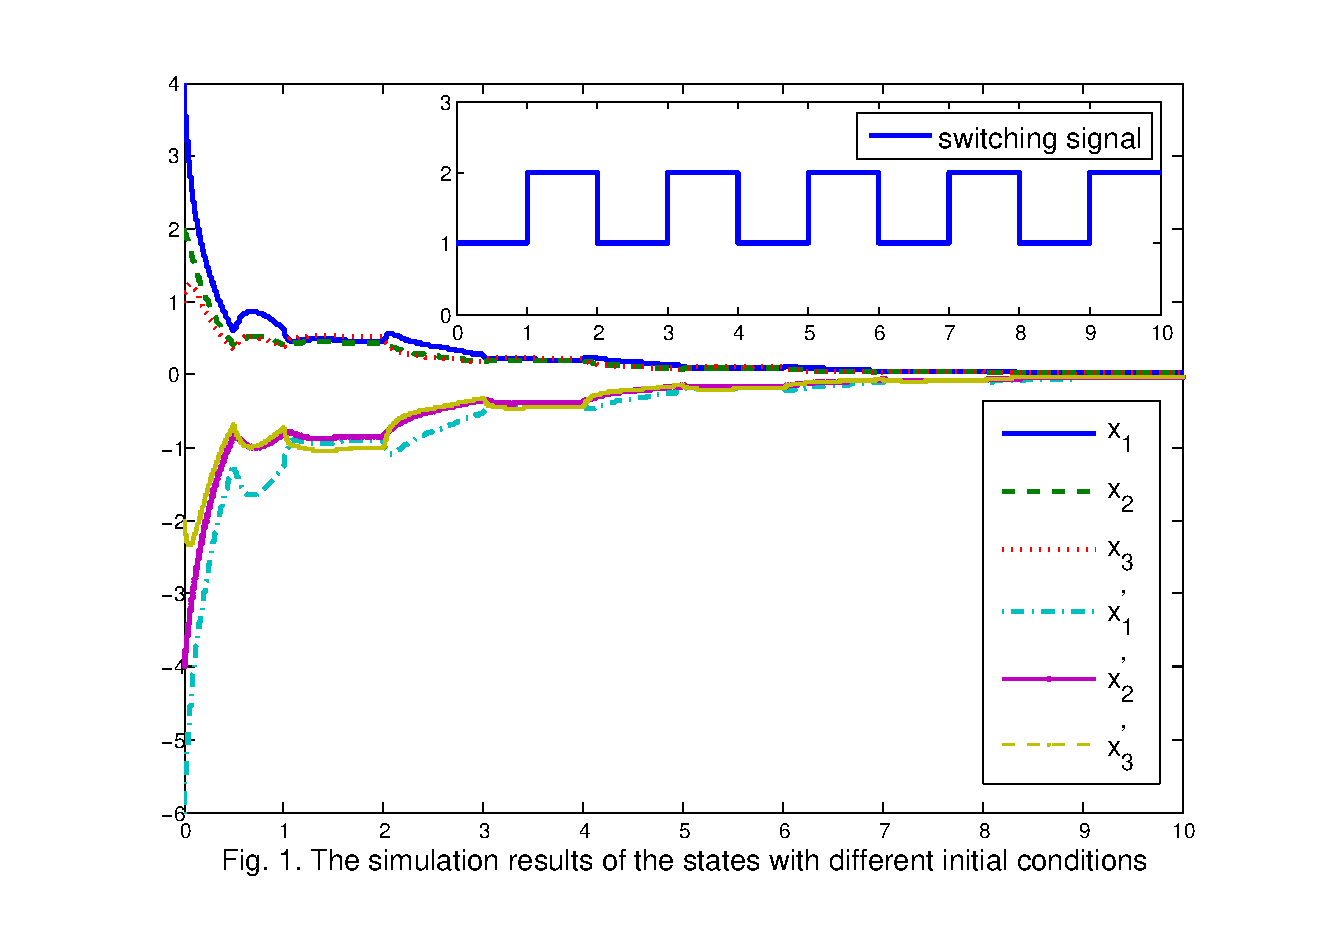
\includegraphics[width=0.45\linewidth]{Figure1}
  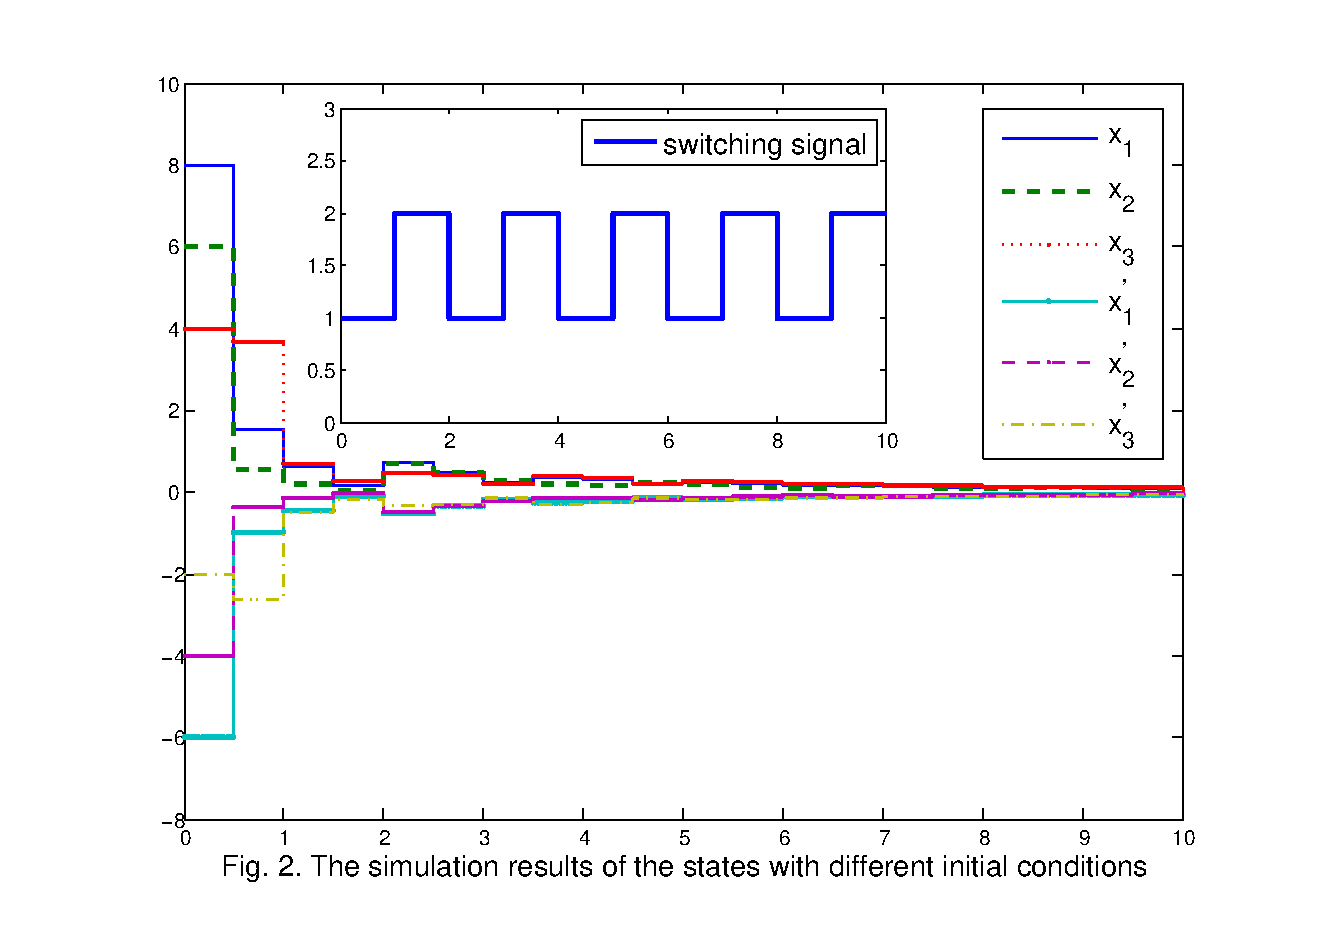
\includegraphics[width=0.45\linewidth]{Figure2}
\end{center}
\vspace{1mm}}

%--------------------------------------------------------------------------------------------------------------------
%	Tables
%--------------------------------------------------------------------------------------------------------------------
\headerbox{Tables}{name=tables,span=2,column=1,below=figures}{
\setlength{\parindent}{1.5em} All tables must be centered in the column and numbered consecutively in Arabic numbers. Table headings should be
placed above the table, as given in Table 1.\vspace{1mm}}

%--------------------------------------------------------------------------------------------------------------------
%	Conclusion
%--------------------------------------------------------------------------------------------------------------------
\headerbox{Conclusion}
{name=conclusion,span=2,column=1,below=tables}{
\setlength{\parindent}{1.5em} One should note that this is only a template for the CCC2016 poster, and the number of the block can be modified freely based on the arrangement of your paper. It is suggested that poster authors use the given poster template, however, the authors are also encouraged to make their personalized posters. No matter what template is used, the format requirements in this template
should be strictly followed.\\
\setlength{\parindent}{1.5em} We would like to stress again that if your paper does not present in the conference, your paper would not be arranged in the programming book.\vspace{1mm}}

%--------------------------------------------------------------------------------------------------------------------
%	References (Change of the reference should go to file sample.bib included in CCC2016_LaTex_poster)
%--------------------------------------------------------------------------------------------------------------------
\headerbox{References}{name=References,span=2,column=1,below=conclusion,bottomaligned=Acknowledgement}{
\renewcommand{\section}[2]{\vskip 0.05em} % Get rid of the default "References" section title
\nocite{*}
\small{
\bibliographystyle{unsrt}
\bibliography{sample} % Use sample.bib as the bibliography file. Change of the reference should go to file sample.bib included in CCC2016_LaTex_poster.
}
\textbf{References} should be listed by order and the reference items are represented as Arabic numbers in square brackets. The authors can decide whether the references section is included or not, however, only key references are required.\\
\setlength{\parindent}{3.5em} It should be note that change of the references should go to the file $sample.bib$ included in the decompressed file  CCC2016-LaTex-poster. The edit of $sample.bib$ can be performed by either the Latex software or Notebook of the computer.\vspace{1mm}}
\end{poster}

\end{document}
\grid
